\section{Comparison}
\label{section:comparison}

\par Now a comparison between the theoretical analysis and the experimental analysis results is done and the results discussed conserning its accuracy and discrepancy. For the theoretical analysis as seen in the previous section a 
 

\begin{figure}[H]
\centering
\begin{subfigure}{.5\textwidth}
  \centering
  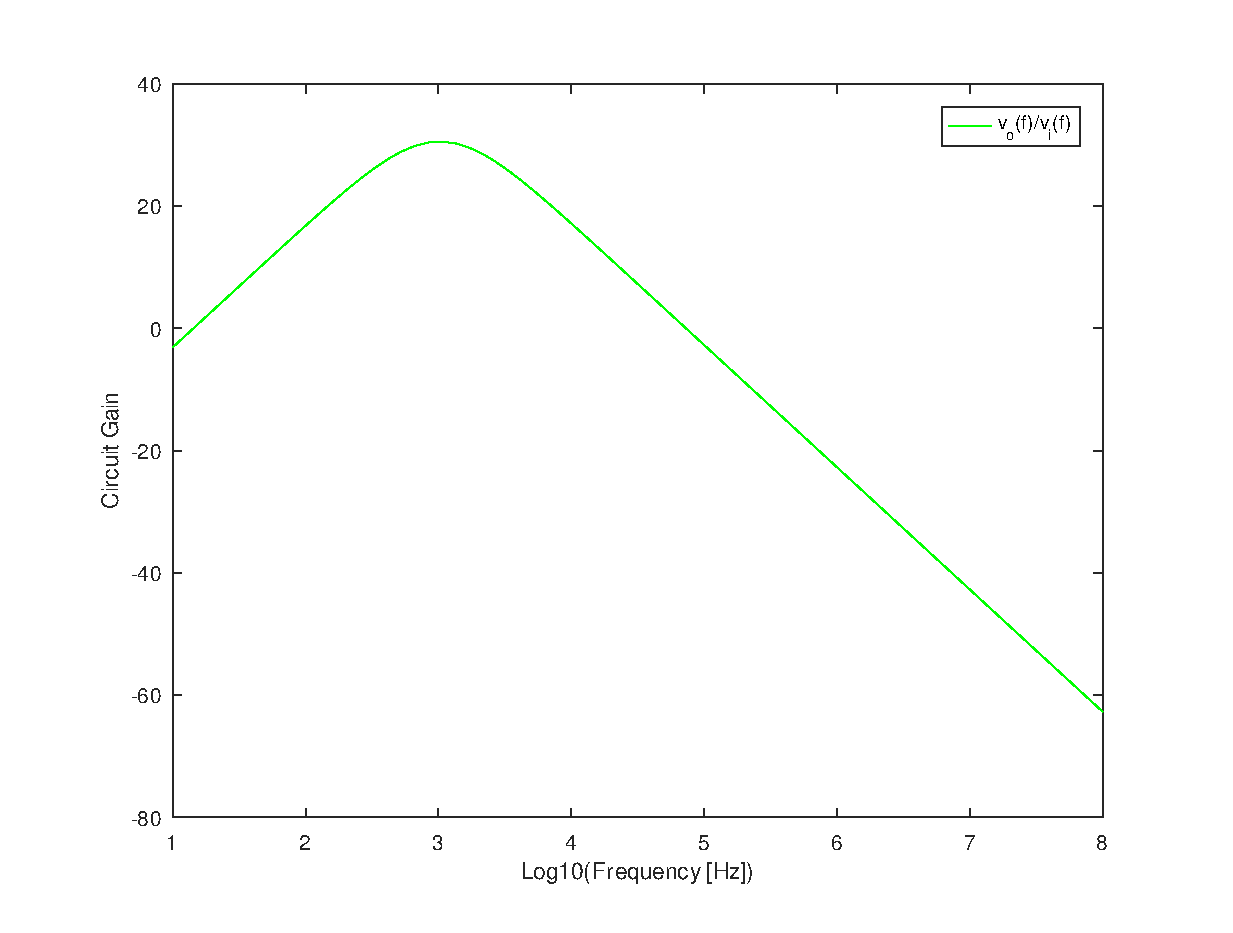
\includegraphics[width=1.1\linewidth]{teoria.eps}
  \caption{Output Voltage - Theoretical Model}
  \label{fig:sim4}
\end{subfigure}
\begin{subfigure}{.5\textwidth}
  \centering
  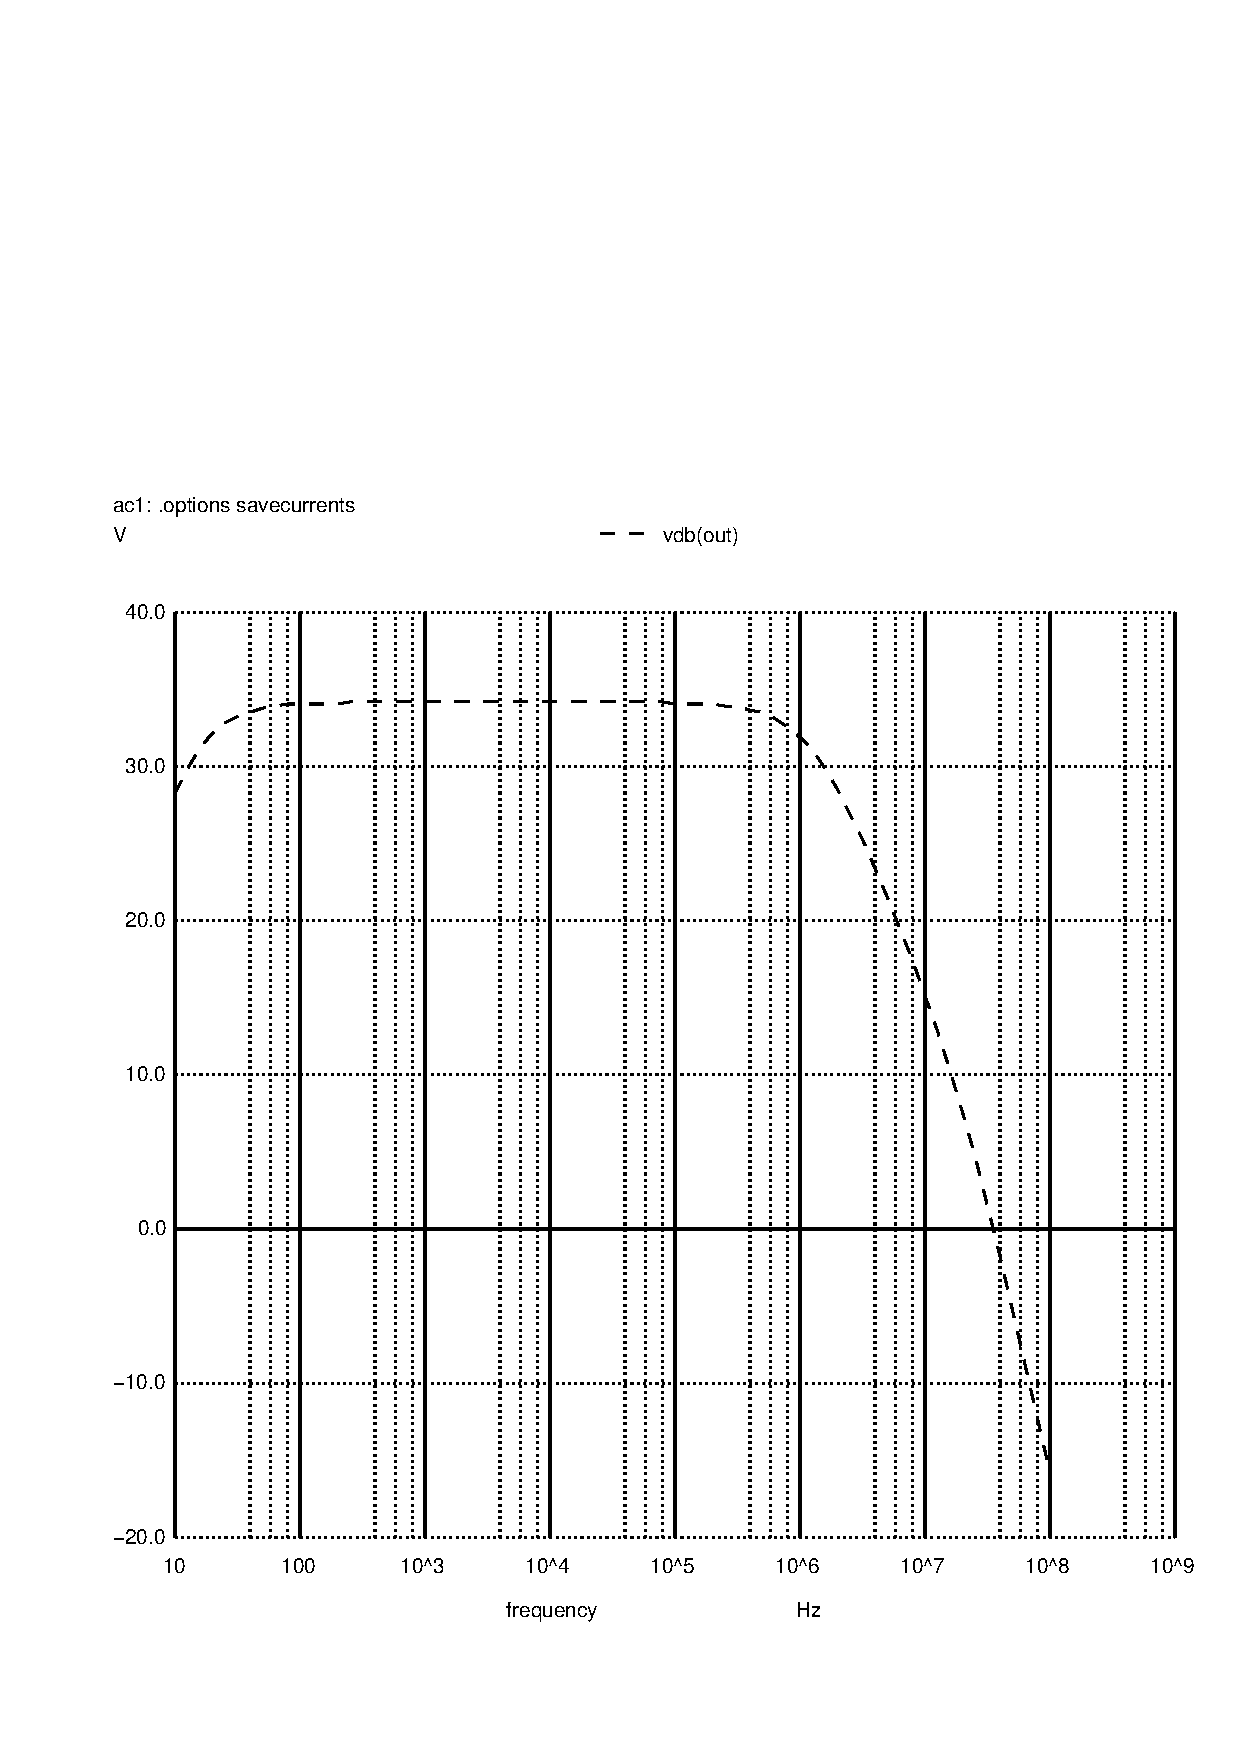
\includegraphics[width=1.1\linewidth]{vo2f.pdf}
  \caption{Output voltage - Ngspice model}
  \label{fig:sim5}
\end{subfigure}
\end{figure}

\par As we can see the graphics are pretty similar, which means that our theoretical model is a good approximation to the real running of an audio amplifier. Furthermore we can compare the values which we are studying and trying to improve: maximum gain and bandwidth and also a comparison between the operating point values is going to be made. The values are shown in the table below.

\begin{table}[H]
\parbox{.45\linewidth}{
  \centering
  \begin{tabular}{|l|r|}
    \hline    
    {\bf Calculus} & {\bf Value [V]} \\ \hline
    @cb[i] & 0.000000e+00\\ \hline
@ce[i] & 0.000000e+00\\ \hline
@q1[ib] & 7.022567e-05\\ \hline
@q1[ic] & 1.404513e-02\\ \hline
@q1[ie] & -1.41154e-02\\ \hline
@q1[is] & 5.765392e-12\\ \hline
@rc[i] & 1.411536e-02\\ \hline
@re[i] & 1.411536e-02\\ \hline
@rf[i] & 7.022567e-05\\ \hline
@rs[i] & 0.000000e+00\\ \hline
v(1) & 0.000000e+00\\ \hline
v(2) & 0.000000e+00\\ \hline
base & 2.254108e+00\\ \hline
coll & 5.765392e+00\\ \hline
emit & 1.411536e+00\\ \hline
vcc & 1.000000e+01\\ \hline

  \end{tabular}
  \caption{Operating point - DC model (V) (Ngspice)}} 
\parbox{.45\linewidth}{
 \centering
  \begin{tabular}{|l|r|}
    \hline    
    {\bf Name} & {\bf Value [V]} \\ \hline
    \input{../mat/ponto0_TAB}
  \end{tabular}
  \caption{Operating point - DC model (V) (Octave)}}
\end{table}

\par As we can see the values are close and the differences that exist may be explained because of the approximations done in the transistor models.
\newpage

